\documentclass[pdf]{beamer}

\mode<presentation>{
  \usetheme{Singapore}          % others: default Singapore Warsaw
  \usecolortheme{dolphin}       % beetle beaver orchid whale dolphin
  \setbeamertemplate{sections/subsections in toc}[ball unnumbered]  % others: circle ball square
	\usepackage{graphicx}
  \graphicspath{ {figures/} }
  \usepackage{listings}
  \lstset{
    basicstyle=\scriptsize\color{blue},
    frame=none,
    columns=l,
    tabsize=2,
    showspaces=false,
    showtabs=false
  }
  \usepackage{array}
  \hypersetup{
    colorlinks=true,
    allcolors=blue
  }
  \usepackage[edges]{forest}
}

% preamble
\title{Ansible Filters}
\subtitle{a short introduction}
\author{Frank Jung}
\institute{frankhjung@linux.com}
\date{ \today }
\logo{ 
\includegraphics[height=1.5cm]{logos.png} }

\begin{document}

\begin{frame}
  \titlepage{}
\end{frame}

% \begin{frame}{Contents}
%   \tableofcontents{}
% \end{frame}

\begin{frame}
  \frametitle{Topics}
  What we will cover \ldots
  \pause{}
  \begin{itemize}
    \item<+-> what are Ansible filters?
    \item<+-> some typical use cases
    \item<+-> getting help
    \item<+-> how to roll my own?
  \end{itemize}
\end{frame}

\section{What are Ansible Filters?}

\begin{frame}
  \frametitle{What are Ansible Filters?}
  Filters are from a fast, flexible, Python template engine called \ldots
  \pause{}
  \begin{center}
    \begin{figure}
      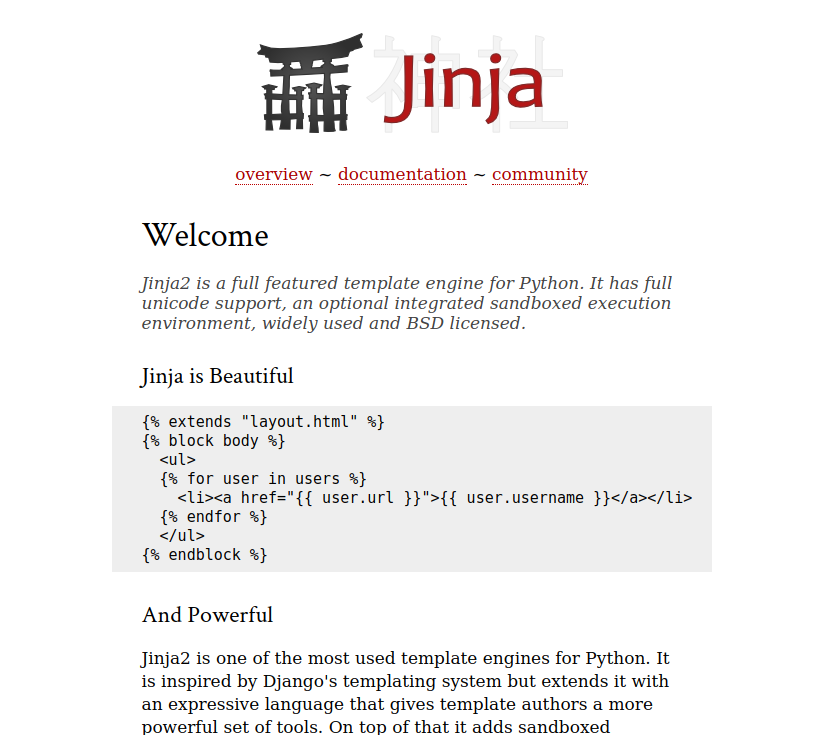
\includegraphics[width=0.5\textwidth]{jinja.png}
    \end{figure}
    \href{http://jinja.pocoo.org}{jinja.pocoo.org}
  \end{center}
\end{frame}

\begin{frame}
  \frametitle{What are Ansible Filters?}
  Filters are used to transform data \ldots
  \pause{}
  \setbeamercolor{alerted text}{fg=blue}
  \begin{enumerate}
    \item<+-> {they can be used inside a template expression}
    \item<+-|alert@+(1)> {they can be used to manipulate local data}
    \item[]
  \end{enumerate}
\end{frame}

\begin{frame}
  \frametitle{What are Ansible Filters?}
  Some important features of filters \ldots
  \pause{}
  \begin{enumerate}
    \item<+->{sand boxed}
      \begin{itemize}
        \item<+->{so can be used to evaluate untrusted code}
      \end{itemize}
    \item<+->{they are executed on the Ansible controller}
      \begin{itemize}
        \item<+->{\textcolor{red}{\textbf{not}} on the task's target host}
      \end{itemize}
    \item<+->{Ansible ships with its own filters}
      \begin{itemize}
        \item<+->{or use standard filters from Jinja2}
        \item<+->{or write your own!}
      \end{itemize}
  \end{enumerate}
\end{frame}

\section{Typical Use Cases}

\begin{frame}[t,fragile]
  \frametitle{Typical Filter Use Cases}
  \only<1-> {Use filters to manipulate local data \ldots \newline}
  \only<2>  {\-\ \color{blue}{\small$\bullet$} create new facts}
  \only<2>  {\lstinputlisting[firstline=34,lastline=36]{filter-examples.yaml}}
  \only<3-> {\-\ \small{\color{blue}$\bullet$} create new facts \newline}
  \only<3>  {\-\ \color{blue}{\small$\bullet$} subset or filter lists}
  \only<3>  {\lstinputlisting[firstline=52,lastline=62]{filter-examples.yaml}}
  \only<4-> {\-\ \small{\color{blue}$\bullet$} subset or filter lists \newline}
  \only<4>  {\-\ \color{blue}{\small$\bullet$} manipulate strings}
  \only<4>  {\lstinputlisting[firstline=87,lastline=99]{filter-examples.yaml}}
\end{frame}

\section{Help}

\begin{frame}[fragile]
  \frametitle{Getting help when things go wrong}
  New in Ansible 2.3 is \verb type_debug :
  \begin{lstlisting}
- name: type_debug var
  debug:
    msg: "{{ martin | type_debug }}"
  \end{lstlisting}
  \pause{}
  Gives variable type information \dots
  \begin{lstlisting}
TASK [type_debug var] *************************
ok: [localhost] => {
    "msg": "dict"
}
  \end{lstlisting}
\end{frame}

\begin{frame}[fragile]
  \frametitle{Getting help when things go wrong}
  Ansible Project - Google Groups
  \begin{center}
    \begin{figure}
      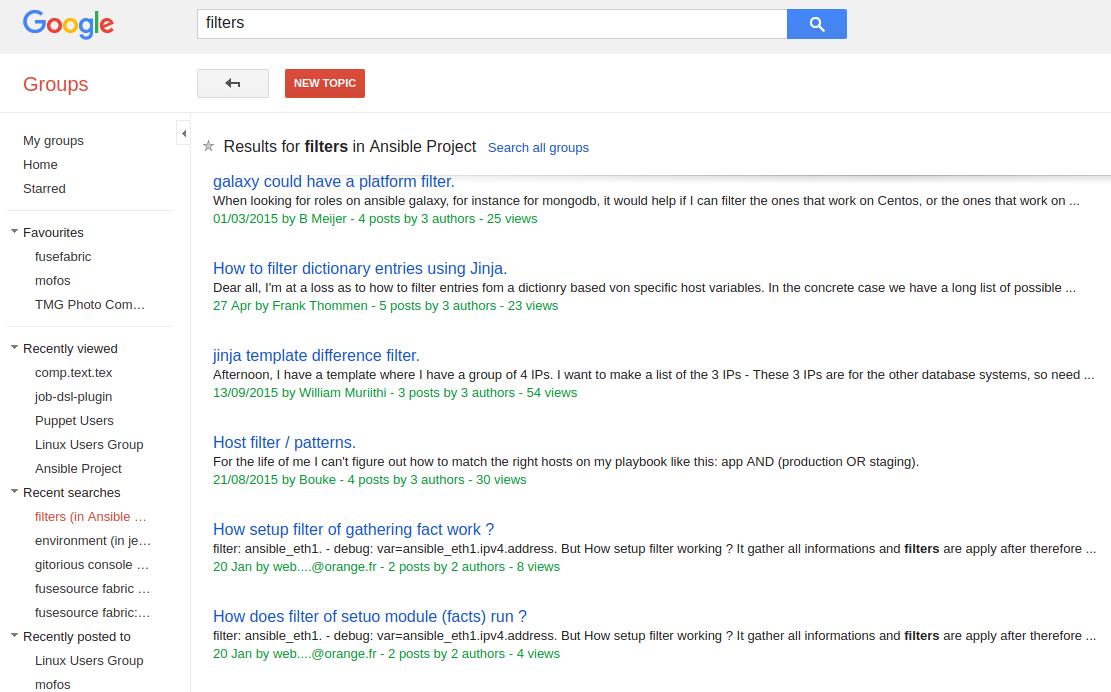
\includegraphics[width=0.8\textwidth]{ansible-google-group.png}
    \end{figure}
  \end{center}
  \tiny \url{https://groups.google.com/d/forum/ansible-project}
\end{frame}

\begin{frame}[t,fragile]
  \frametitle{Getting help when things go wrong}
  Read the source, for example Jinja has a sort method:
  \begin{lstlisting}[title=\tiny\url{https://github.com/pallets/jinja/blob/master/jinja2/filters.py}, captionpos=b]
def do_sort(environment, value, reverse=False,
            case_sensitive=False, attribute=None):
    """Sort an iterable.  Per default it sorts ascending,
    if you pass it true as first argument it will reverse
    the sorting.
    ...
  \end{lstlisting}
  \pause{}
  Where \texttt{do\_sort} maps to \ldots \pause{} \textit{sort}:
  \begin{lstlisting}
FILTERS = {
  ...
    'sort':                 do_sort,
  ...
}
  \end{lstlisting}
  \pause{}
  Which gives a hint on how to use this method:
  \begin{lstlisting}
- name: sort skills
  debug:
    var: item
  with_items: "{{ martin.skills | sort(reverse=True) }}"
  \end{lstlisting}
\end{frame}

\section{Roll Your Own}

\begin{frame}
  \frametitle{Writing your own filter}
  \begin{itemize}[<+->]
    \item[] You may think to start here \ldots
      \begin{itemize}
        \item<1->
          \small \url{http://docs.ansible.com/ansible/dev_guide/developing_plugins.html}
      \end{itemize}
    \item[]
      But, that only redirects you to
      \href{https://github.com/ansible/ansible/blob/devel/lib/ansible/plugins/filter/core.py}{lib/ansible/plugins/filter} \ldots
    \item[] A better place to start is \ldots
      \begin{itemize}
        \item
          \href{https://opensolitude.com/2016/05/21/ansible-jinja2-filter-plugins.html}{Enhance
          your Ansible playbooks with custom Jinja2 filters} \newline
        \small \url{https://opensolitude.com/2016/05/21/ansible-jinja2-filter-plugins.html}
      \end{itemize}
    \item[] Let's go through an example in detail \ldots
  \end{itemize}
\end{frame}

\begin{frame}[t,fragile]
  \frametitle{Writing your own filter}
  To create a custom filter the steps are \ldots
  \begin{itemize}[<+->]
    \item {write a test for your plugin}
    \item {create a directory called \color{blue}{\texttt{filter\_plugins}}}
    \item {add a Python script into this directory, to this script \ldots}
      \begin{itemize}
        \item {add a function implementing your filter}
        \item {implement class \textcolor{blue}{\texttt{FilterModule}} overriding \textcolor{blue}{\texttt{filters}} method}
      \end{itemize}
    \item {run test on your new filter}
  \end{itemize}
\end{frame}

\begin{frame}[t,fragile]
  \frametitle{Writing your own filter}
  Writing a custom filter in detail \ldots
  \setbeamercolor{normal text}{fg=gray}
  \setbeamercolor{alerted text}{fg=blue}
  \usebeamercolor{normal text}
  \begin{itemize}
    \item \alert {write a test for your plugin \texttt{example.yaml}}
      \begin{lstlisting}
- name: count number of occurrences of 'r' in name
  set_fact: counter="{{ martin.name | count('r') }}"

- name: test there are exactly 2 occurrences
  debug: var=counter
  failed_when: counter | int != 2
      \end{lstlisting}
    \item {create a directory called \texttt{filter\_plugins}}
    \item {add a Python script into this directory, to this script \ldots}
      \begin{itemize}
        \item {add a function implementing your filter}
        \item {implement class \texttt{FilterModule} overriding \texttt{filters} method}
      \end{itemize}
    \item {run test on your new filter}
  \end{itemize}
\end{frame}

\begin{frame}[t,fragile]
  \frametitle{Writing your own filter}
  Writing a custom filter in detail \ldots
  \setbeamercolor{normal text}{fg=gray}
  \setbeamercolor{alerted text}{fg=blue}
  \usebeamercolor{normal text}
  \begin{itemize}
    \item {write a test for your plugin}
    \item \alert {create a directory called \texttt{filter\_plugins}}
      \begin{lstlisting}
mkdir filter_plugins
      \end{lstlisting}
    \item {add a Python script into this directory, to this script \ldots}
      \begin{itemize}
        \item {add a function implementing your filter}
        \item {implement class \texttt{FilterModule} overriding \texttt{filters} method}
      \end{itemize}
    \item {run test on your new filter}
  \end{itemize}
\end{frame}

\begin{frame}[t,fragile]
  \frametitle{Writing your own filter}
  Writing a custom filter in detail \ldots
  \setbeamercolor{normal text}{fg=gray}
  \setbeamercolor{alerted text}{fg=blue}
  \usebeamercolor{normal text}
  \begin{itemize}
    \item {write a test for your plugin}
    \item {create a directory called \texttt{filter\_plugins}}
    \item \alert {add a Python script into this directory \ldots}
      \begin{lstlisting}
touch filter_plugins/custom.py
      \end{lstlisting}
      \begin{itemize}
        \item {add a function implementing your filter}
        \item {implement class \texttt{FilterModule} overriding \texttt{filters} method}
      \end{itemize}
    \item {run test on your new filter}
  \end{itemize}
\end{frame}

\begin{frame}[t,fragile]
  \frametitle{Writing your own filter}
  \setbeamercolor{normal text}{fg=gray}
  \setbeamercolor{alerted text}{fg=blue}
  \usebeamercolor{normal text}
  Writing a custom filter in detail \ldots
  \begin{itemize}
    \item {write a test for your plugin}
    \item {create a directory called \texttt{filter\_plugins}}
    \item {add a Python script into this directory, to this script \ldots}
      \begin{itemize}
        \item \alert {add a function implementing your filter}
          \begin{lstlisting}
def count(word, char):
  return word.count(char)
          \end{lstlisting}
        \item {implement class \texttt{FilterModule} overriding \texttt{filters} method}
      \end{itemize}
    \item {run test on your new filter}
  \end{itemize}
\end{frame}

\begin{frame}[t,fragile]
  \frametitle{Writing your own filter}
  \setbeamercolor{normal text}{fg=gray}
  \setbeamercolor{alerted text}{fg=blue}
  \usebeamercolor{normal text}
  Writing a custom filter in detail \ldots
  \begin{itemize}
    \item {write a test for your plugin}
    \item {create a directory called \texttt{filter\_plugins}}
    \item {add a Python script into this directory, to this script \ldots}
      \begin{itemize}
        \item {add a function implementing your filter}
        \item \alert {implement class \texttt{FilterModule} overriding \texttt{filters} method}
          \begin{lstlisting}
class FilterModule(object):
  def filters(self):
      return {'count': count}
          \end{lstlisting}
      \end{itemize}
    \item {run test on your new filter}
  \end{itemize}
\end{frame}

\begin{frame}[fragile]
  \frametitle{Writing your own filter}
  Resulting Ansible project structure \ldots
  \color{blue}
  \begin{center}
    \begin{forest}
      for tree={%
        folder,
        grow'=0,
        fit=band,
      }
      [.
        [ansible.cfg]
        [filter-examples.yaml]
        [filter\_plugins
          [custom.py]
        ]
        [hosts]
        [README.md]
      ]
    \end{forest}
  \end{center}
\end{frame}

\begin{frame}[t,fragile]
  \frametitle{Writing your own filter}
  \setbeamercolor{normal text}{fg=gray}
  \setbeamercolor{alerted text}{fg=blue}
  \usebeamercolor{normal text}
  Writing a custom filter in detail \ldots
  \begin{itemize}
    \item {write a test for your plugin}
    \item {create a directory called \texttt{filter\_plugins}}
    \item {add a Python script into this directory, to this script \ldots}
      \begin{itemize}
        \item {add a function implementing your filter}
        \item {implement class \texttt{FilterModule} overriding \texttt{filters} method}
      \end{itemize}
    \item \alert {run test on your new filter}
  \end{itemize}
\end{frame}

\section{Summary}

\begin{frame}
  \frametitle{What we covered \ldots}
    \pause{}
  \begin{itemize}[<+->]
    \item{what filters are}
    \item{typical places you will use them}
    \item{getting help when things go wrong}
    \item{writing your own filter}
  \end{itemize}
\end{frame}

\begin{frame}
  \frametitle{References}
  \begin{itemize}
    \item
      \href{https://github.com/frankhjung/ansible-filters}{Presentation and sample code}
      \begin{itemize}
        \item \url{https://github.com/frankhjung/ansible-filters}
      \end{itemize}
    \item
      \href{https://www.ansible.com/}{www.ansible.com}
      \begin{itemize}
        \item \href{http://docs.ansible.com/ansible/playbooks_filters.html}{filters}
        \item \href{https://github.com/ansible/ansible}{github} - \url{https://github.com/ansible/ansible}
      \end{itemize}
    \item
      \href{https://groups.google.com/d/forum/ansible-project}{Ansible Project - Google Groups}
    \item
      \href{http://jinja.pocoo.org/}{jinja.pocoo.org}
      \begin{itemize}
        \item \href{http://jinja.pocoo.org/docs/2.9/templates}{filters}
        \item \href{https://github.com/pallets/jinja}{github} - \url{https://github.com/pallets/jinja}
      \end{itemize}
    \item
      \href{https://opensolitude.com/2016/05/21/ansible-jinja2-filter-plugins.html}{Enhance your Ansible playbooks with custom Jinja2 filters}
      \begin{itemize}
        \item \url{https://opensolitude.com/2016/05/21/ansible-jinja2-filter-plugins.html}
      \end{itemize}
  \end{itemize}
\end{frame}

\begin{frame}
  \frametitle{Addendum}
  \begin{tabular}{ m{1cm} m{6cm} }
    
\includegraphics[width=1.0cm]{ansible-logo.png} & Ansible \\
    
\includegraphics[width=1.0cm]{acm-logo.png} & Association for Computing Machinery \\
    
\includegraphics[width=1.0cm]{thelinuxfoundation-logo.png} & The Linux Foundation \\
    
\includegraphics[width=1.0cm]{themarlogroup-logo.png} & The Marlo Group
  \end{tabular}
\end{frame}

\end{document}
